% This part of the document is the "Preamble" - everything before your main document.
% It includes any authorship info, as well as formatting, packages, and additional 
% things needed to produce the document. Essentially, almost everything except 
% actual content.

\documentclass{article} 	% Identifies what kind of document you are working on
%\documentclass[twocolumn]{article}

\usepackage{geometry, amsmath, bm, hyperref, graphicx, authblk}
\hypersetup{colorlinks=true, linkcolor=blue, urlcolor=blue, citecolor=blue}
\numberwithin{equation}{section}
\title{Learning \LaTeX}
\author[1]{Matthew Frenkel}
\author[2]{Donna Wrublewski}
\author[1]{John Doe}
\author[1,*]{John Smith}
\affil[1]{NYU}
\affil[2]{Caltech}
\affil[*]{ASCE}
\newcommand{\tensor}[1]{\bar{\bar{#1}}}		% Creates a tensor command

\begin{document}			% Starts document/ends preamble
	\maketitle
	\newpage
	\tableofcontents
	\newpage

	\section{Introduction}
	\LaTeX{} is a typesetting tool that allows for easy use of mathematical equations, as well as better control of formatting.  In this introduction we will examine the critical structures in \LaTeX{}, as well as some of its most common commands.  For more information please visit the Caltech \LaTeX{} \href{http://libguides.caltech.edu/latex}{guide}.

	\section{Tips Before Getting Started}
	Before you start writing your \LaTeX document there are a few things you should consider.  First make sure you create a folder for the document you are creating and place any images, figures, or bibliographical information inside that folder.  This will make your life much easier as you import this items into your document.
	%\section{Tips Before Getting Started}
	Before you start writing your \LaTeX document there are a few things you should consider.  First make sure you create a folder for the document you are creating and place any images, figures, or bibliographical information inside that folder.  This will make your life much easier as you import this items into your document.

	\section{Parts of a LaTeX Document}
	A standard \LaTeX{} document will have 2 different sections, the \textbf{preamble} and \textbf{body}.  The \textbf{bibliography} can be considered a third section but it is not required of all \LaTeX{} documents.

		\subsection{Preamble}
	The preamble is the first part of a \LaTeX{} document.  It will be used to call packages for the document and to define parameters of both the document and its packages where needed.  The preamble will always begin with the command \verb|\documentclass{}| and end with the command \verb|\begin{document}|.

		\subsection{Body}
	The body of a \LaTeX{} document can is where the content will go.  The document body will begin with the command \verb|\begin{document}| and end with the command \verb|end{document}|.

	\section{\LaTeX{} structures and environments}
	There are several important structures and environments that are critical to building a \LaTeX{} environment.  In this section we will take about \textbf{commands}, \textbf{text}, \textbf{packages}, \textbf{comments}, and \textbf{math}.

		\subsection{Commands}
		Commands are structures within \LaTeX{} that are read by the compiler and instruct it to take a certain action.  Commands can range in purpose from inserting a symbol such as \verb|\pi| $\pi$ to creating complicated structures like tables or matrices.  Command always start with a \verb|\|.  Commands can have a few different formats but generally a command will have the following structure \verb|\command[option argument]{required}|.

		Commands are case sensitive and generally speaking will end at a point of punctuation or number.  For example take a look at what happens if I type \verb|\pi9| $\pi9$.

		There are also many commands in \LaTeX{} that use the form \verb|\begin{argument}| it is very important to remember that all of these commands must have a corresponding \verb|\end{argument}| or there will be an error when you compile.  Some common commands like this are \verb|\begin{document}|, \verb|\begin{equation}|, \verb|\begin{matrix}|, and \verb|\begin{tabular}|.

		\subsection{Text}
		Text is easy to input in \LaTeX{}.  Once inside of the body of your document text can be entered and will be compiled.  Commands can be used to format and adjust text.  A new paragraph can be entered by living a blank space in the source document.

		Some commone text commands are \verb|\textbf{}| \textbf{for boldface}, \verb|\textit{}| \textit{for italics}, \verb|\Large| \Large for large\normalsize, \verb|\tiny| \tiny for tiny\normalsize, and \verb|\emph{}| \emph{for emphasis}.

		\subsection{Packages}
		Package belong in the preamble.  They are used to import additional features into a \LaTeX{} document.  To call a package use the command \verb|\usepackage{}|.

		\subsection{Comments}
		Comments can be include in a document by using the \% symbol.  The compiler will ignore anything that follows the \%.

		\subsection{Math}
		Math is a very important environment with \LaTeX.  It is what allows equations to be easily written and to be visual appealing.  But, \LaTeX must be told that it is in a math environment to display properly and to use certain commands.  Take for example the following equation:\\
		\\
		2sin(x)=y \\
		$2\sin(x)=y$\\
		\\
		An immediate difference can be seen in the way that the mathematics is displayed.

		This simplest way to display math is to use \$ to surround the mathematical text.  A \$ will active the math environment until another \$ appears.  This is useful for writing in line math.  For example I can place the equation $2\sin(x)=y$.  You should also note that certain commands can only be used in math mode for example if I want to insert the $\pi$ symbol I need to be in a math environment.

		Another useful mathematical environment is display mode.  This can be started by using the command \verb|\[| and ended using the command \verb|\]|.  The display mode is helpful for taking math outside of a line of text for example: \[2\sin(x)=y\] can be written using display mode, and I don't need to do anything extra to create the spacing or centering.

		Another method for displaying mathematics is to use a command that creates a mathematical environment such as \verb|\begin{equation}| or \verb|\begin{align}|.  Notice what happens if I use \verb|\begin{equation}|:
		\begin{equation}
			2\sin(x)=y \\
		\end{equation}
		See how there is now an equation number.  If you want to have more than one equation in a single begin and end you should use the\verb|\begin{align}| environment.  In this environment you can also use the \& to visual control your equations and the \verb|\\| to start a new line.  For example:
		\begin{align}
			2\sin(x)&=y \\
			3\cos(x)e^{i\pi x}&=y
		\end{align}
		These two equations are aligned using a \& before the equals sign.

		The mathematical environment in \LaTeX{} is very powerful and easily capable of creating very advanced equations with a little practice:
		\begin{align} 				% Enters math mode/equation mode/display mode use & or && for aligning
		\vec{\nabla} \cdot \vec{E} \quad &=\quad\frac{\rho}{\epsilon_{0}} &&\text{Gauss's Law} \label{eq:GL}\\  	%labels allow you to reference back to the equation in your text
		\vec{\nabla} \cdot \vec{B} \quad &=\quad 0 &&\text{Gauss's Law for Magnetism} \label{eq:GLM}\\
		\vec{\nabla} \times \vec{E} \quad &=\hspace{10pt}-\frac{\partial{\vec{B}}}{\partial{t}} &&\text{Faraday's Law of Induction} \label{eq:FL}\\
		\vec{\nabla} \times \vec{B} \quad &=\quad \mu_0 \left( \epsilon_0\frac{\partial{\vec{E}}}{\partial{t}}+\vec{J} \right) &&\text{Ampere's Circuital Law} \label{eq:AL}
		\end{align}
		\begin{align}
		\tensor{\epsilon} &= \begin{matrix} % \tensor is our user defined command and bmatrix creates a braketed matrix
			\epsilon_{11} && \epsilon_{12} &&\epsilon_{13} \\
			\epsilon_{21} && \epsilon_{22} &&\epsilon_{23} \\
			\epsilon_{31} && \epsilon_{32} &&\epsilon_{33} \\
		\end{matrix}
		\label{eq:matrix}  % label of equation
		\end{align}
		\begin{equation}
		F(x)= A_0 + \sum_{n=1}^N\left[ A_n\cos{\left(\frac{2\pi nx}{P}\right)}+B_n\sin{\left(\frac{2\pi nx}{P}\right)}\right]
		\end{equation}
		Also note that you can label equations by using the command \verb|\label{label}|.  This is helpful if you want to reference back to the equation later on using the command \verb|\ref{label}|.  For example \ref{eq:matrix}.
	\section{Tables}
	There are two commands that are useful for creating tables.  The most important one is\verb|\begin{tabular}{columns}| the second is \verb|\begin{table}[location]|.  The first of these two commands allows you to create a the visual table.  The second allows you to tell \LaTeX{} that you are creating a table so that you can better control how it is format within the larger document.  Here is an example of a simple table:
	\begin{table}[h]
		\caption{a simple table}
		\centering
		\begin{tabular}{|cc|l|r|}
			\hline
			centered & centered & left & right \\
			\hline
			$1$ & $x=y$&$\pi$&$\Pi$\\
			\hline
		\end{tabular}
	\end{table}

	\section{Graphics}
	Figures are added to a document by including the graphix package in the preamble \verb|\usepackage{graphix}|. A figure environment is started with the command \verb|\begin{figure}[location]|.  The figure (\ref{fig:workshop_image}) is loaded with the command \verb|\includegraphics[keyvals]{imagefile}|, it is important to note that the ``imagefile'' must be located inside the same folder as the .tex file.
	\begin{figure}[htb]			% h=here, b=bottom, t=top, ! stress this
		\centering
		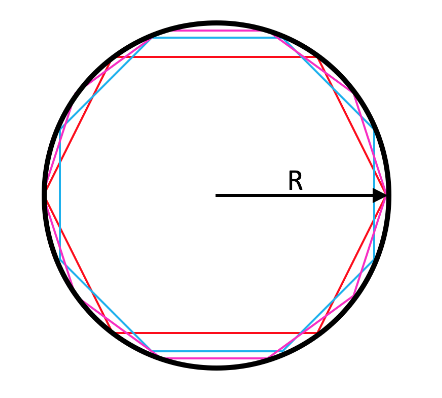
\includegraphics[width=.4\textwidth]{workshop_image}
		\caption{Different resonance conditions of light in circular cavity} \cite{frenkel_fine_2013}  \label{fig:workshop_image}
	\end{figure}

	\section{Bibliography}
	Bibliographies can be made directly using commands in \LaTeX{} or the can be made using a bib\TeX{} file as done here.  To create the bibliography use the command \verb|\bibliography{filename}|, to set the style use the command \verb|\bibliographystyle|, and to cite something use the command \verb|\cite{bibID}| \cite{frenkel_-chip_2016}.
	\bibliographystyle{ieeetr}
	\bibliography{latex_workshop_bib_file}
\end{document}
